\section{流体与催化剂颗粒外表面的传质与传热}


\begin{frame}
    \frametitle{流体与催化剂颗粒外表面的传质}

    多相催化反应过程的第一步是反应物向催化剂颗粒外表面传递，这一步骤的速率可用下式来表示
    \[
        N_{\mathrm{A}} =k_{\mathrm{G}} a_{\mathrm{m}}(c_{\mathrm{AG}}-c_{\mathrm{AS}})
    \]
    式中$a_{\mathrm{m}}$为单位质量催化剂颗粒的外表面积，$k_{\mathrm{G}}$为传质系数。
    
    浓度差$(c_{\mathrm{AG}}-c_{\mathrm{AS}})$为传质过程推动力。
    
    对于定态过程，这一传质速率应等于反应物A的转化速率$-\mathscr{R}_{\mathrm{A}}$，即
    \[
        N_{\mathrm{A}} = -\mathscr{R}_{\mathrm{A}}
    \]

\end{frame}


\begin{frame}
    \frametitle{流体与催化剂颗粒外表面的传热}

    由于化学反应进行时总是伴随着一定的热效应，放热或吸热，因而在反应物向催化剂颗粒外表面传递的同时，必然产生流体与颗粒外表面间的热量传递，进行放热反应时，热量从催化剂外表面向流体主体传递，吸热反应则相反，此传热速率可用下式表示
    \[
        q = h_{\mathrm{s}} a_{\mathrm{m}}(T_{\mathrm{s}}-T_{\mathrm{G}})
    \]
    式中$h_{\mathrm{s}}$为流体与颗粒外表面间的传热系数；$T_{\mathrm{s}}$及$T_{\mathrm{G}}$则分别表示颗粒外表面和流体主体的温度，此温度差为传热推动力。过程达到定态时传热量应等于反应放出（或吸收）的热量，即
    \[
        q =(-\mathscr{R}_{\mathrm{A}})(-\Delta H_{\mathrm{r}})
    \]

\end{frame}


\begin{frame}
    \frametitle{传递系数}

    上述两个传递方程中都包含传递系数，即传质系数$k_{\mathrm{G}}$和传热系数$h_{\mathrm{s}}$。
    
    传递系数反映了传递过程阻力的大小，实质上也就是围绕催化剂颗粒外表面上层流边界层的厚薄。温度差和浓度差产生于层流边界层的两侧。
    
    处理实际的相间传递问题时，通常做如下假设：
    \begin{itemize}
        \item 颗粒外表面上温度均一，浓度也均一。
        \item 流体主体温度和浓度也均一。
    \end{itemize}
    这实质上是假定层流边界层的厚度处处相等，这样的假设将相间传递问题作为一维问题来处理，使复杂的问题大为简化而又保持足够的近似。
    
\end{frame}


\begin{frame}
    \frametitle{传递系数}

    传递阻力的大小对于传递速率的影响至关重要，阻力越大则传递系数越小。流体与固体颗粒间的传质系数与颗粒的几何形状及尺寸、流体力学条件以及流体的物理性质有关。影响流体与颗粒间传热系数的因素同样是这些。
    
    较为普遍采用的实验方法是，用关联传质因子$j_{\mathrm{D}}$和传热因子$j_{\mathrm{H}}$的方法来计算传质系数$k_{\mathrm{G}}$和传热系数$h_{\mathrm{s}}$。
    \[
        j_{\mathrm{D}}=\frac{k_{\mathrm{G}} \rho}{G}(S c)^{2 / 3}
    \]
    \[
        j_{\mathrm{H}}=\frac{h_{\mathrm{s}}}{G C_{p}}(P r)^{2 / 3}
    \]
    式中$Sc$和$Pr$分别为施密特数和普朗特数，$G$为气体质量流速，$C_{p}$为气体恒压比热容。
    \[
        S_{c}=\mu / \rho D, \quad P r=C_{p} \mu / \lambda_{\mathrm{f}}
    \]
    式中，$\mu$为气体的粘度，$\rho$为气体密度，$D$为分子扩散系数，$\lambda$为气体导热系数。

\end{frame}


\begin{frame}
    \frametitle{传递系数}

    无论$j_\mathrm{D}$还是$j_\mathrm{H}$，均是雷诺数的函数，其函数形式与床层结构有关。
    
    例如，对于固定床
    \[
        \varepsilon j_{\mathrm{D}}=0.357 / R e^{0.359}
    \]
    上式应用范围为$3 \ll Re \ll 1000$，$0.6 \ll Sc \ll 5.4$。
    \[
        \varepsilon j_{\mathrm{H}}=0.395 / R e^{0.36}
    \]
    应用范围$0.6 \ll Re \ll 3000$，$30 \ll Sc \ll 10^5$。

    上两式中的雷诺数均系按颗粒的直径来定义，即
    \[
        R e=d_{\mathrm{p}} G / \mu
    \]
    根据传热与传质的类比原理有
    \[
        j_{\mathrm{D}}=j_{\mathrm{H}}
    \]

\end{frame}


\begin{frame}
    \frametitle{传递系数}

    由$j_{\mathrm{D}}$与$Re$的关联式$\varepsilon j_{\mathrm{D}}=0.357 / R e^{0.359}$可知，传质系数$k_\mathrm{G}$将随质量速度$G$的增长而变大，从而也就加快了外扩散传质速率；反之，质量速度下降，外扩散传质阻力变大，甚至会成为过程的控制步骤。

    实际生产中，在条件允许的前提下，力求用较大的质量速度以提高设备的生产强度，故属于外扩散控制的气固催化反应过程不多。
    
    硝酸生产中的铂网催化剂上的氨氧化反应属于外扩散控制，原因有二:
    \begin{itemize}
        \item 反应温度高达800、900℃，本征反应速率很快，
        \item 加大氨空气混合气的质量速度会招致铂网的机械摩擦损失增加。
    \end{itemize}

\end{frame}


\begin{frame}
    \frametitle{流体与颗粒外表面间的浓度差和温度差}

    气固相催化反应，过程达到定态时传热量等于反应放出（或吸收）的热量
    \[
        k_{\mathrm{G}} a_{\mathrm{m}}(c_{\mathrm{AG}}-c_{\mathrm{AS}})(-\Delta H_{\mathrm{r}})=h_{\mathrm{s}} a_{\mathrm{m}}(T_{\mathrm{S}}-T_{\mathrm{G}})
    \]
    将传质$j$因子$j_\mathrm{D}$和传热$j$因子$j_\mathrm{H}$代入，整理后得
    \[
        T_{\mathrm{S}}-T_{\mathrm{G}}=(c_{\mathrm{AG}}-c_{\mathrm{AS}}) \frac{(-\Delta H_{\mathrm{r}})}{\rho {C}_p}\left(\frac{P r}{S c}\right)^{2 / 3}\left(\frac{j_{\mathrm{D}}}{j_{\mathrm{H}}}\right)
    \]
    就多数气体而言，${P r}/{S c} \approx 1$，对于固定床，$j_\mathrm{D}$与$j_\mathrm{H}$近似相等，于是
    \[
        T_{\mathrm{S}}-T_{\mathrm{G}}=\frac{(-\Delta H_{\mathrm{r}})}{\rho{C_p}}(c_{\mathrm{AG}}-c_{\mathrm{AS}})
    \]
    由此可见，催化剂外表面与流体主体的温度差和浓度差成线性关系。

\end{frame}


\begin{frame}
    \frametitle{外扩散对多相催化反应的影响(单一反应)}

    为了说明外扩散对多相催化反应的影响，引用外扩散有效因子$\eta_\mathrm{X} $，其定义为
    \[
        \eta_\mathrm{X} = \frac{\text{外扩散有影响时颗粒外表面处的反应速率}}{\text{外扩散无影响时颗粒外表面处的反应速率}}
    \]
    显然，颗粒外表面上的反应物浓度总是低于气相主体的浓度，因此
    \begin{itemize}
        \item 反应级数为正，则$\eta_\mathrm{X} \leqslant 1$；
        \item 反应级数为负，则$\eta_\mathrm{X} \geqslant 1$。
    \end{itemize}

    下面只讨论颗粒外表面与气相主体间不存在温度差且粒内也不存在内扩散阻力时的情况，即只考虑相间传质，而不考虑相间传热和内扩散的影响。

\end{frame}


\begin{frame}
    \frametitle{外扩散对多相催化反应的影响(单一反应)}

    对于一级不可逆反应，
    \[
        \eta_{\mathrm{X}}=\frac{k_{\mathrm{W}} c_{\mathrm{AS}}}{k_{\mathrm{W}} c_{\mathrm{AG}}}=\frac{c_{\mathrm{AS}}}{c_{\mathrm{AG}}} 
    \]
    对于定态过程
    \[
        k_{\mathrm{G}} a_{\mathrm{m}}(c_{\mathrm{AG}}-c_{\mathrm{AS}})=k_{\mathrm{W}} c_{\mathrm{AS}}
    \]
    解得
    \[
       c_{\mathrm{AS}}=c_{\mathrm{AG}} /(1+D a) \qquad \text{式中，} D a=k_{\mathrm{W}} / k_{\mathrm{G}} a_{\mathrm{m}}
    \]
    一级不可逆反应的外扩散有效因子
    \[
        \eta_{\mathrm{X}}=1 /(1+D a)
    \]
    $D a$称丹克莱尔数，是化学反应速率与外扩散速率之比，当$k_{\mathrm{W}}$一定时，此值越小，$k_{\mathrm{G}} a_{\mathrm{m}}$越大，即外扩散影响越小。

\end{frame}


\begin{frame}
    \frametitle{外扩散对多相催化反应的影响(单一反应)}

    对于$\alpha$级不可逆反应，其丹克莱尔数
    \[
        D a=k_{\mathrm{W}} c_{\mathrm{AG}}^{a-1} /(k_{\mathrm{G}} a_{\mathrm{m}})
    \]
    不同反应级数时的$\eta_{\mathrm{X}}$值为
    \[
        \alpha=2 \quad \eta_{\mathrm{X}}=\frac{1}{4 D a^{2}}(\sqrt{1+4 D a}-1)^{2} \qquad  \qquad \qquad \quad 
    \]

    \[
        \alpha=\frac{1}{2} \quad \eta_{\mathrm{X}}=\left[\frac{2+D a^{2}}{2}\left(1-\sqrt{1-\frac{4}{(2+D a^{2})^{2}}}\right)\right]^{1 / 2}
    \]

    \[
        \alpha=-1 \quad \eta_{\mathrm{X}}=2 /(1+\sqrt{1-4 D a}) \qquad  \qquad \qquad \qquad \quad 
    \]

\end{frame}



\begin{frame}
    \frametitle{外扩散对多相催化反应的影响(单一反应)}

    \begin{minipage}{0.58\linewidth}
        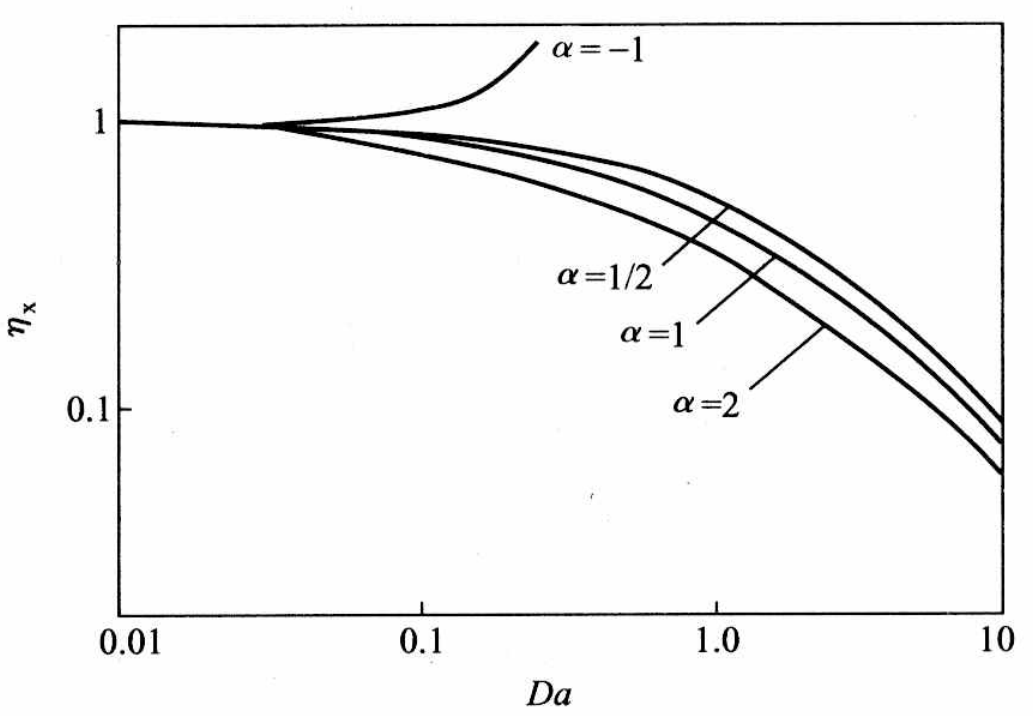
\includegraphics[width=\linewidth]{figures/fig6.2.png}
    \end{minipage}\hfill
    \begin{minipage}{0.4\linewidth}
        \begin{itemize}
            \item 除反应级数为负外，外扩散有效因子总是随丹克莱尔数的增加而降低；
            \item $\alpha$越大，外扩散有效因子随$Da$增加而下降得越明显；
            \item 无论$\alpha$为何值：$Da$趋于零时，$\eta_{\mathrm{X}}$总是趋于1。
        \end{itemize}
    \end{minipage}

    \bigskip
    反应级数越高，就越有必要采取措施降低外扩散阻力，以提高外扩散有效因子。

\end{frame}


\begin{frame}
    \frametitle{外扩散对多相催化反应的影响(平行反应)}

    考虑颗粒外表面与气相主体温度相同时的情况：
    \[
        \ch{A -> B} \qquad r_\mathrm{B} = k_1c_\mathrm{AS}^ \alpha
    \]
    \[
        \ch{A -> D} \qquad r_\mathrm{D} = k_2c_\mathrm{AS}^ \beta
    \]
    由反应瞬时选择性的定义可写出
    \[
        S = r_\mathrm{B}/(r_\mathrm{B} + r_\mathrm{D}) = 1/(1 + k_2 c_\mathrm{AS}^{\beta - \alpha}/k_1)
    \]
    如外扩散阻力甚小以致对过程无明显影响，则$c_\mathrm{AS} = c_\mathrm{AG}$，此时的瞬时选择性为
    \[
        S' = r_\mathrm{B}/(r_\mathrm{B} + r_\mathrm{D}) = 1/(1 + k_2 c_\mathrm{AG}^{\beta - \alpha}/k_1)
    \]

\end{frame}


\begin{frame}
    \frametitle{外扩散对多相催化反应的影响(平行反应)}

    比较以上二式可知，外扩散对于平行反应选择性的影响，取决于$\beta - \alpha$是正还是负
    \begin{itemize}
        \item 若$\alpha > \beta$，则$S < S'$
        
        外扩散影响的存在，使生成目的产物B的选择性降低，这是因为，外扩散阻力的存在，使得$c_\mathrm{AS} < c_\mathrm{AG}$，当生成目的产物B的反应级数大于副反应的反应级数时，外扩散阻力对主反应的影响程度大于对副反应的影响，故生成B的选择性下降；
        \item 若$\alpha < \beta$，则$S = S'$
        
        外扩散影响的存在，使生成目的产物B的选择性升高；
        \item 若$\alpha = \beta$，则$S = S'$
        
        外扩散不影响目的产物B的选择性。
    \end{itemize}

\end{frame}


\begin{frame}
    \frametitle{外扩散对多相催化反应的影响(连串反应)}

    对于一级不可逆连串反应
    \[
        \ce{A ->[k_1] B ->[k_2] D}
    \]
    B为目的产物，假设A、B和D的传质系数均相等，当过程为定态时可写出
    \[
        \begin{array}{l}
            k_{\mathrm{G}} a_{\mathrm{m}}\left(c_{\mathrm{AG}}-c_{\mathrm{AS}}\right)=k_{1} c_{\mathrm{AS}} \\
            k_{\mathrm{G}} a_{\mathrm{m}}\left(c_{\mathrm{BS}}-c_{\mathrm{BG}}\right)=k_{1} c_{\mathrm{AS}}-k_{2} c_{\mathrm{BS}} \\
            k_{\mathrm{G}} a_{\mathrm{m}}\left(c_{\mathrm{DS}}-c_{\mathrm{DG}}\right)=k_{2} c_{\mathrm{BS}}
            \end{array}
    \]
    由以上各式可得
    \[
        c_{\mathrm{AS}}=c_{\mathrm{AG}} /\left(1+D_{a 1}\right)
    \]
    \[
        c_{\mathrm{B}_{\mathrm{S}}}=\frac{D_{\mathrm{a} 1} c_{\mathrm{AG}}}{\left(1+D_{\mathrm{a} 1}\right)\left(1+D_{\mathrm{a} 2}\right)}+\left(\frac{c_{\mathrm{BG}}}{1+D_{\mathrm{a} 2}}\right)
    \]
    式中，$D_{\mathrm{a} 1}=k_{1} / k_{\mathrm{G}} a_{\mathrm{m}}, D_{\mathrm{a} 2}=k_{2} / k_{\mathrm{G}} a_{\mathrm{m}} $。

\end{frame}


\begin{frame}
    \frametitle{外扩散对多相催化反应的影响(连串反应)}

    反应的瞬时选择性
    \[
        S=\left(k_{1} c_{\mathrm{AS}}-k_{2} c_{\mathrm{BS}}\right) / k_{1} c_{\mathrm{AS}}=1-\frac{k_{2} D_{\mathrm{a} 1}}{k_{1}\left(1+D_{\mathrm{a} 2}\right)}-\frac{k_{2} c_{\mathrm{BG}}\left(1+D_{\mathrm{a} 1}\right)}{k_{1} c_{\mathrm{AG}}\left(1+D_{\mathrm{a} 2}\right)}
    \]
    由$D_{\mathrm{a} 1}$和$D_{\mathrm{a} 2}$的表达式可知
    \[
        D_{\mathrm{a} 2} = k_2 D_{\mathrm{a} 1}/k_1
    \]
    代入$S$表达式可得
    \[
        S=\frac{1}{1+D_{\mathrm{a} 2}}-\frac{k_{2} c_{\mathrm{BG}}\left(1+D_{\mathrm{a} 1}\right)}{k_{1} c_{\mathrm{AG}}\left(1+D_{\mathrm{a} 2}\right)} 
    \]
    当$D_{\mathrm{a} 1} = D_{\mathrm{a} 2} = 0$，即外扩散对过程没有影响时，上式变为
    \[
        S^{\prime}=1-k_{2} c_{\mathrm{BG}} / k_{1} c_{\mathrm{AG}}
    \]

\end{frame}


\begin{frame}
    \frametitle{外扩散对多相催化反应的影响(连串反应)}
    \[
        S^{\prime}=1-\frac{k_{2} c_{\mathrm{BG}}}{k_{1} c_{\mathrm{AG}}} 
    \]
    \[
        S=\frac{1}{1+D_{\mathrm{a} 2}}\left[ 1-\frac{k_{2} c_{\mathrm{BG}}\left(1+D_{\mathrm{a} 1}\right)}{k_{1} c_{\mathrm{AG}}} \right]
    \]
    外扩散阻力的存在，使连串反应的选择性降低，这是与平行反应不同之处。
    
    因此，对于连串反应，需设法降低外扩散阻力，以提高反应的选择性。
    
    例如萘氧化制苯酐、苯氧化制顺酐等氧化反应，需力求降低外扩散阻力，以避免深度氧化，从而增加目的产物的收率。

    若颗粒外表面与气相主体间，由于传热阻力而\bf{存在温度差}，如前所述，对于放热反应一般是$T_\mathrm{S} > T_\mathrm{G}$，这时，对复合反应选择性的影响决定于各反应的活化能。

\end{frame}


\begin{frame}[t]
    \frametitle{}

    \begin{example}
        \ce{A ->[k_1] B ->[k_2] D}为一级不可逆放热连串反应，已知$T_\mathrm{G} = \SI{450}{K}$，$c_\mathrm{BG}/c_\mathrm{AG} = 0.5$，$(T_\mathrm{S} - T_\mathrm{G}) = \SI{10}{K}$，$(k_\mathrm{G}a_\mathrm{m})_\mathrm{A} = (k_\mathrm{G}a_\mathrm{m})_\mathrm{B} = \SI{40}{cm^3/(g.s)}$，$k_1 = \num{6.0e8} \exp{[-E_1/RT]}$，\si{cm^3/(g.s)}，$k_2 = \num{1.2e6} \exp{[-E_2/RT]}$，\si{cm^3/(g.s)}，$E_1 = \SI{80.0}{kJ/mol}$，$E_2 = \SI{60.0}{kJ/mol}$。试求反应选择性。
    \end{example}
    \only<2>{
    \begin{itemize}
        \item[1.] 只考虑浓度差不考虑温度差
    \end{itemize}
        $T_\mathrm{S} = T_\mathrm{G} = \SI{450}{K}$

        $k_1 = \SI{0.310}{cm^3/(g.s)}$，$k_2 = \SI{0.130}{cm^3/(g.s)}$

        $D_\mathrm{a1} = 0.310/40 = \num{7.75e-3}$，$D_\mathrm{a2} = 0.130/40 = \num{3.25e-3}$

        考虑外扩散影响，$S = \frac{1}{1 + 3.25 \times 10^{-3}} - \frac{0.130(1 + 7.75 \times 10^{-3})0.5}{0.310(1 + 3.25 \times 10^{-3})} = 0.786$

        不考虑外扩散影响，$S' = 1 - 0.130 \times 0.5/0.310 = 0.790$
        }
        \only<3>{
            \begin{itemize}
                \item[2.] 同时考虑气相与颗粒外表面的浓度差与温度差
            \end{itemize}
            \[            
                T_\mathrm{S} =  \SI{460}{K},\qquad k_1 = \SI{0.494}{cm^3/(g.s)},\qquad  k_2 = \SI{0.184}{cm^3/(g.s)} 
            \]
            \[
                D_\mathrm{a1} = 0.01235,\qquad  D_\mathrm{a2} = 0.0046 
            \]
            \[
                S = \frac{1}{1 + 0.0046} - \frac{0.184(1.01235)0.5}{0.494(1.0046)} = 0.8077
            \]
        }
        \only<4>{
            
            \begin{itemize}
                \item[3.] 只考虑颗粒表面温度差，不考虑浓度差
            \end{itemize}
        不考虑外扩散影响，
        \[
            S'' = 1 - 0.184 \times 0.5/0.494 = 0.8138
        \]
        }
        

\end{frame}


\begin{frame}
    \frametitle{外扩散对多相催化反应的影响(连串反应)}

    \begin{itemize}
        \item $T_\mathrm{S} = T_\mathrm{G}$
        
        外扩散阻力的影响，总是使连串反应的选择性降低
        \item 放热反应，$T_\mathrm{S} > T_\mathrm{G}$
            \begin{itemize}
                \item[\bullet] 主反应活化能>副反应活化能
                
                选择性$S$比$S''$小，比$S'$大
                \item[\bullet] 主反应活化能<副反应活化能
            \end{itemize}
    \end{itemize}
\end{frame}


\begin{frame}[t]
    \frametitle{}

    \begin{example}
        在半径为R的球形催化剂上，等温进行气相反应\ch{A <=> B}。试以A或B的浓度为纵坐标，径向距离$r$为横坐标，针对下列三种情况分别绘出A和B的浓度分布示意图。
    
    （1）化学动力学控制

    （2）外扩散控制

    （3）内、外扩散的影响均不能忽略

    \end{example}

\end{frame}